\documentclass{purdue-slide}

% For filler text:
\usepackage[base]{babel}
\usepackage{lipsum}
\usepackage{lmodern}
\usepackage{pgfplots}
\usepackage{caption}
\usepackage{tikz}
\usetikzlibrary{positioning}

% For non-CS Purdue logo use the lines below:
% \renewcommand{\titlelogo}{\includesvg[width=.3\paperwidth,keepaspectratio]{logo/pu-rev.svg}}
% \renewcommand{\slidelogo}{\includesvg[width=.3\paperwidth,keepaspectratio]{logo/pu.svg}}
% You can also request a logo from https://marcom.purdue.edu/toolbox/logos/

\title{A Purdue \LaTeX\ Slide Template}
\subtitle{Made with Beamer}
\author{A Purdue Student\texorpdfstring{\footnotemark[1]}{}, A Duepur Student\texorpdfstring{\footnotemark[2]}{}}
\renewcommand{\slidefoot}{\LaTeX\ Template}

\begin{document}

\begin{titleframe}{}
	\maketitle
\end{titleframe}

\begin{frame}{Contents}
	% \textbf{Introduction to Linear Programming} \\
	% \textbf{Mathematical Theory \& Theorems} \\
	% \textbf{Introduction to PuLP} \\
	% \textbf{Case Studies} \\
	% \textbf{Resources \& References} \\
	\tableofcontents
\end{frame}

\section{Theoretical Foundation}

\begin{frame}{Fundamental Theorem of LP}
	\textbf{Theorem:} If a linear programming (LP) problem is feasible and bounded, then it has an optimal solution.
\end{frame}

\begin{frame}{Proof of the Theorem}
	Without loss of generality, we may assume that the LP problem is of the form:
	\[
		\begin{aligned}
			& \min \mathbf{c}^\top \mathbf{x} \\
			(P) \quad & \text{s.t. } A\mathbf{x} \geq \mathbf{b}
		\end{aligned}
	\]
	where $m$ and $n$ are positive integers,  $A \in \mathbb{R}^{m \times n}, \ \mathbf{b} \in \mathbb{R}^m, \mathbf{c} \in \mathbb{R}^n,$ $ \text{ and }
	\mathbf{x} =
	\begin{bmatrix}
		x_1 \\
		\vdots \\
		x_n
	\end{bmatrix} \text{ is a tuple of variables. }$

\end{frame}

\begin{frame}{Transforming to Standard Form}
	\quad Any LP problem can be converted to the standard form $(P)$ having the same feasible region and optimal solution set.

	For this, note that:

	\begin{itemize}
		\item Constraints of the form $\mathbf{a}^\top \mathbf{x} \leq \beta$ become $-\mathbf{a}^\top \mathbf{x} \geq -\beta$
		\item Constraints of the form  $\mathbf{a}^\top \mathbf{x} = \beta$ become:
			\[
    \mathbf{a}^\top \mathbf{x} \geq \beta \quad \text{and} \quad -\mathbf{a}^\top \mathbf{x} \leq -\beta
			\]
		\item Maximization problems become minimizations of $-\mathbf{c}^\top \mathbf{x}$
	\end{itemize}
\end{frame}

\begin{frame}{Auxiliary System}
	Suppose $(P)$ is feasible. Define an auxiliary system:
	\[
		(S) \quad
		\begin{cases}
			z - \mathbf{c}^\top \mathbf{x} \geq 0 \\
			-z + \mathbf{c}^\top \mathbf{x} \geq 0 \\
			A\mathbf{x} \geq \mathbf{b}
		\end{cases}
	\]

	\vspace{0.5em}
	Solving $(P)$ is equivalent to minimizing $z$ in $(S)$.

	\vspace{0.5em}
	We eliminate variables $x_1, \dots, x_n$, reducing $(S)$ to a system $(S')$ involving only $z$.
\end{frame}

\begin{frame}{Boundedness and Optimal Solution}
	If $(P)$ is bounded, then $(S')$ must include the constraints:
	\[
		z \geq \beta_i \text{, where } \beta_i \in \mathbb{R}, \forall  i = 1, \dots, p, \text{ with } p \in \mathbf{N^*}.
	\]
	Define $\gamma = \max\{\beta_1, \dots, \beta_p\}$. Then for any solution $x, z$ to $(S)$, $z$ is at least $\gamma$. But we can set $z = \gamma$ and extend it to a solution for $(S)$.

	Hence, we obtain an optimal solution for $(P)$ and $\gamma$ is the optimal value. This completes the proof of the theorem.
\end{frame}

\begin{frame}{ Multipliers and the Inequality}
	$\mathbf{Remark:}$ We can construct multipliers to derive the inequality:
	\[
		\mathbf{c}^\top \mathbf{x} \geq \gamma
	\]
	from the system $A\mathbf{x} \geq \mathbf{b}$.

	There exist real values $\alpha, \beta, y_1^*, \ldots, y_m^* \geq 0$ such that:
	\[
		\left[ \alpha \ \beta \ y_1^* \cdots y_m^* \right]
		\begin{bmatrix}
			1 & -\mathbf{c}^\top \\
			-1 & \mathbf{c}^\top \\
			0 & A
		\end{bmatrix}
		\begin{bmatrix}
			z \\ \mathbf{x}
		\end{bmatrix}
		\geq
		\left[ \alpha \ \beta \ y_1^* \cdots y_m^* \right]
		\begin{bmatrix}
			0 \\ 0 \\ \mathbf{b}
		\end{bmatrix}
	\]
\end{frame}

\section{Hand-written examples}

\begin{titleframe}{Hand-written Examples}

\end{titleframe}

\begin{frame}{LP Problem: Maximize Workshop Profit}
	A workshop produces:
	\begin{itemize}
		\item Desks: 4h woodworking, 2h painting, \$40 profit
		\item Chairs: 3h woodworking, 1h painting, \$25 profit
	\end{itemize}

	Available resources:
	\begin{itemize}
		\item 24 hours of woodworking
		\item 10 hours of painting
	\end{itemize}

	\textbf{Goal:} Maximize profit by choosing how many desks and chairs to build.
\end{frame}

\begin{frame}{LP Formulation}
	Let:
	\begin{itemize}
		\item \(x\): number of desks
		\item \(y\): number of chairs
	\end{itemize}

	\textbf{Maximize: } \(Z = 40x + 25y\)

	\textbf{Subject to:}
	\[
		\begin{aligned}
			4x + 3y &\leq 24 \quad \text{(woodworking)} \\
			2x + y &\leq 10 \quad \text{(painting)} \\
			x, y &\geq 0
		\end{aligned}
	\]
\end{frame}

\begin{frame}{LP Solution by Hand: Find Intersection}
	\textbf{Find where constraints intersect:}

	\[
		\begin{aligned}
			4x + 3y &= 24 \\
			2x + y &= 10 \Rightarrow y = 10 - 2x
		\end{aligned}
	\]

	Substitute into the first equation:

	\[
		4x + 3(10 - 2x) = 24 \Rightarrow 4x + 30 - 6x = 24 \Rightarrow -2x = -6 \Rightarrow x = 3
	\]

	Then:

	\[
		y = 10 - 2(3) = 4
	\]

	\textbf{Intersection point: } \((3, 4)\)
\end{frame}

\begin{frame}{LP Solution by Hand: Evaluate Z}
	\textbf{Corner points:}
	\begin{itemize}
		\item \((0, 8)\): \(Z = 0 + 25 \times 8 = 200\)
		\item \((5, 0)\): \(Z = 40 \times 5 + 0 = 200\)
		\item \((3, 4)\): \(Z = 40 \times 3 + 25 \times 4 = 220\) ✅
	\end{itemize}

	\begin{alertblock}{Optimal Solution}
		\(x = 3\), \(y = 4\); Max profit = \textbf{\$220}
	\end{alertblock}
\end{frame}

% Plot
\begin{frame}{Feasible Region: LP - Workshop}
	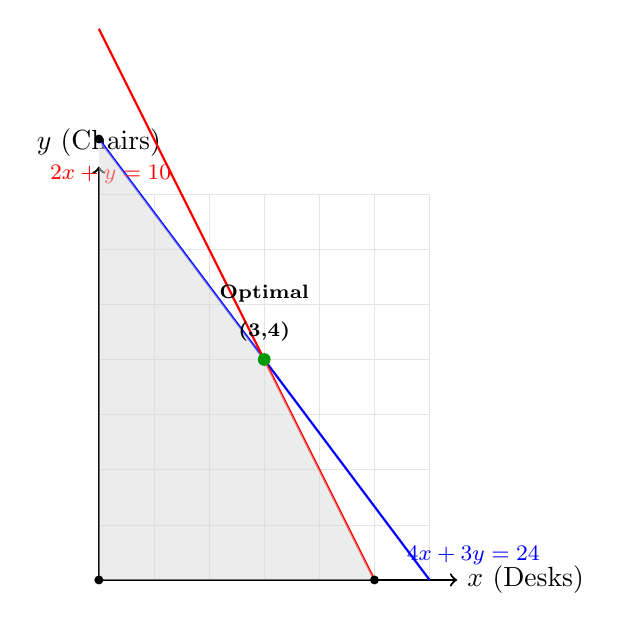
\begin{tikzpicture}[scale=0.7]
		\draw[very thin, gray!20] (0,0) grid (6,7);

		% Axes
		\draw[->, thick] (0,0) -- (6.5,0) node[right] {$x$ (Desks)};
		\draw[->, thick] (0,0) -- (0,7.5) node[above] {$y$ (Chairs)};

		% Constraint lines with adjusted labels
		\draw[thick, blue] (0,8) -- (6,0)
		node[pos=0.9, below right, text=blue] {\footnotesize $4x + 3y = 24$};
		\draw[thick, red] (0,10) -- (5,0)
		node[pos=0.3, above left, text=red] {\footnotesize $2x + y = 10$};

		% Feasible region (shaded)
		\fill[gray!30, opacity=0.5] (0,0) -- (0,8) -- (3,4) -- (5,0) -- cycle;

		% Points
		\foreach \x/\y in {0/0, 0/8, 3/4, 5/0} {
			\filldraw[black] (\x,\y) circle (2pt);
		}

		\node at (3,4.5) {\scriptsize \textbf{(3,4)}};
		\filldraw[green!60!black] (3,4) circle (3pt);
		\node at (3,5.2) {\scriptsize \textbf{Optimal}};
	\end{tikzpicture}
	\vspace{-1em}
	\captionof{figure}{Feasible region for LP: Maximize \$40x + \$25y}
\end{frame}

\begin{frame}{ILP Problem: Integer Optimization}
	\textbf{Objective:} Maximize \(Z = 3x + 2y\)

	\textbf{Subject to:}
	\[
		\begin{aligned}
			x + y &\leq 4 \\
			2x + y &\leq 5 \\
			x, y &\in \mathbb{Z}_{\geq 0}
		\end{aligned}
	\]

	\textbf{Step 1: Find feasible integer pairs \((x,y)\):}
	\begin{itemize}
		\item Try values: \((0,0)\), \((1,2)\), \((2,1)\), \((1,3)\), etc.
	\end{itemize}

	\textbf{Step 2: Evaluate \(Z = 3x + 2y\)}

	\begin{itemize}
		\item \((1,3) \Rightarrow Z = 9\) ✅
		\item \((2,1) \Rightarrow Z = 8\)
		\item \((0,4) \Rightarrow Z = 8\)
	\end{itemize}

	\begin{alertblock}{Optimal ILP Solution}
		\(x = 1\), \(y = 3\); Max value = \textbf{9}
	\end{alertblock}
\end{frame}

\begin{frame}{ILP Solution by Hand}
	\textbf{Step 1: Generate integer pairs \((x, y)\) that satisfy the constraints.}

	\textbf{Constraints:}
	\[
		\begin{aligned}
			x + y &\leq 4 \\
			2x + y &\leq 5 \\
			x, y &\in \mathbb{Z}_{\geq 0}
		\end{aligned}
	\]

	Try values of \(x\) from 0 to 3:

	\begin{itemize}
		\item \(x = 0\): \(y \leq 4\) and \(y \leq 5\) → \(y = 0,1,2,3,4\)
		\item \(x = 1\): \(y \leq 3\) and \(y \leq 3\) → \(y = 0,1,2,3\)
		\item \(x = 2\): \(y \leq 2\) and \(y \leq 1\) → \(y = 0,1\)
		\item \(x = 3\): \(y \leq 1\) and \(y \leq -1\) → ❌ infeasible
	\end{itemize}

	Total valid integer points:
	\((0,0), (0,1), (0,2), (0,3), (0,4), (1,0), (1,1), (1,2), (1,3), (2,0), (2,1)\)
\end{frame}

\begin{frame}{Feasible Integer Points: ILP}
	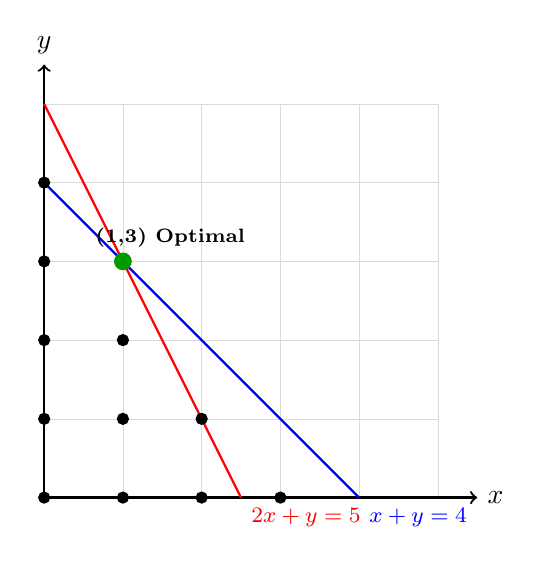
\begin{tikzpicture}[scale=1]
		\draw[very thin, gray!30] (0,0) grid (5,5);

		% Axes
		\draw[->, thick] (0,0) -- (5.5,0) node[right] {$x$};
		\draw[->, thick] (0,0) -- (0,5.5) node[above] {$y$};

		% Constraint lines
		\draw[thick, blue] (0,4) -- (4,0) node[below right] {\footnotesize $x + y = 4$};
		\draw[thick, red] (0,5) -- (2.5,0) node[below right] {\footnotesize $2x + y = 5$};

		% Feasible integer points
		\foreach \x/\y in {
			0/0, 0/1, 0/2, 0/3, 0/4,
			1/0, 1/1, 1/2, 1/3,
			2/0, 2/1,
			3/0
		} {
			\filldraw[black] (\x,\y) circle (2pt);
		}

		% Optimal point
		\filldraw[green!60!black] (1,3) circle (3pt);
		\node at (1.6,3.3) {\scriptsize \textbf{(1,3) Optimal}};
	\end{tikzpicture}
	\captionof{figure}{Feasible integer points for ILP: Maximize \(3x + 2y\)}
\end{frame}

\end{document}